\documentclass[11pt]{report}

	\usepackage[myheadings]{fullpage}


	\usepackage[style=verbose-note,bibstyle=authortitle]{biblatex}
	\bibliography{bibliography}

	\usepackage{graphicx}
	\usepackage{amsmath}
	\usepackage{subfigure}
	\subfiguretopcaptrue

	\usepackage{fancyhdr}
	\usepackage{setspace}
	\setstretch{1.7}

	\bibliography{bibliography}
	\makeatletter
	\renewcommand\@biblabel[1]{}
	\makeatother

	\renewcommand{\figurename}{Example}

	% \newcommand{\footnoteremember}[2]{\footnote{#2}\newcounter{#1}\setcounter{#1}{\value{footnote}}}
	% \newcommand{\footnoterecall}[1]{\footnotemark[\value{#1}]}

	\def\fattitle{``One never knows -- \emph{do} one?''}
	\def\fatslogan{the remarkable gifts of Fats Waller}


	\pagestyle{fancy}
	\rhead{Amiel Martin}
	\lhead{\fattitle{}: \fatslogan}

	\usepackage{titlepic}

	\title{\fattitle \\
		\large \fatslogan}
	\author{Amiel Martin}	
	\date{May 21, 2009}
	\titlepic{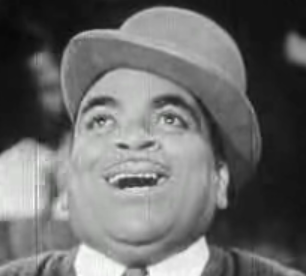
\includegraphics{fats1.png}}
	

\usepackage{graphics}
\begin{document}
	\maketitle

	\label{sec:introduction}
	When Fats Waller was introduced to Billy Kyle, pianist for John Kirby, Waller commented on a recording of theirs he had heard recently. Patting Kyle on the back he said, ``That modulation you play from A-flat to F was simply terrific! Where did you get that one from, man?'' To which Kyle replied, ``I took it off a record of yours.''\footnote{\cite[231]{anecdotes}.} This story, along with many others from \emph{Jazz Anecdotes}, demonstrates a consequence of his impetuous and larger-than-life lifestyle; he very much lived in the moment. In order to support this outsized lifestyle in financially difficult times, Waller turned to comedy, popular music, and high throughput. He was best known for his satirical lyrics and stride style at the piano -- even so, Fats Waller was a more talented musician than he gets credit for.

	\label{sec:piano_skills}
	Thomas Wright ``Fats'' Waller is known as ``the greatest of the Harlem jazz pianists''\footnote{\cite[2]{life}.} and the only stride pianist to become famous because of it.\footnote{\cite[146]{visions}.} Fats had a large range of stylistic capabilities, but by far the most popular was his stride. The term ``stride'' refers to a style of piano playing originated by James P. Johnson and probably derived from the ragtime technique of alternating between low notes and higher chords with the left hand.\footnote{for more about ``stride'', see \cite[79]{experience}.} In \emph{Fats Waller: his Life \& Times}, Alyn Shipton explains that as stride diverged from ragtime, the left-hand parts became more complex and less regular, and the right-hand parts became more complex and difficult as well.\footnote{\cite[5]{life}.} Fats picked up many techniques and prowess from his mentor James P. Johnson and by watching him perform cutting-contests (a form of musical battle in the 1920s-1930s). During that time he also picked up from Johnson ``a love of the classics, a respect for musical literacy, and (so far as the piano was concerned) a taste and delicacy of touch that allowed Fats the full dynamic range in his playing.''\footnote{\cite[8]{life}.}
	
	Waller's stride technique, as he puts it, is ``all in knowing what to put on the right beat''\footnote{quote from \emph{Metronome} 52:2 (February 1936): 33 found in \cite{transcriptions}.}; a steady pulsating bass in the left hand, embellishments in the right hand that are sparse and subservient to the melody, and overall, expression through rising and falling with sudden contrasts to build climaxes.
	
	
		\begin{figure}[ht]
			\centering
			\begin{minipage}{\textwidth}
				
				\caption{excerpt from \emph{My feelin's are hurt} (1929) transcr. B. Dobbens.\protect\footnote{\scriptsize From \cite[]{grove-book:waller}.}}
				\label{fig:hurt}
				

				{%
\parindent 0pt
\ifx\preLilyPondExample \undefined
\else
  \expandafter\preLilyPondExample
\fi
\def\lilypondbook{}%
\input b4/lily-d03c2438-systems.tex
\ifx\postLilyPondExample \undefined
\else
  \expandafter\postLilyPondExample
\fi
}


			\end{minipage}
		\end{figure}

	Fats was exceptional at improvising over classic stride. He also augmented the standard 2 beat stride rhythm with occasional three-beat cross-rhythms. These rhythms are exemplified in Example~\ref{fig:hurt}, along with many of his other standard style traits, such as his tasteful variety of tone and texture (a skill he probably developed as an organ player), and the chromatic alterations and added inner pitches to octaves and 10\textsuperscript{ths} in the left hand that were undoubtedly a large influence to Art Tatum (another stride pianist, and one of the few who could rival Waller's mastery in technique).\footnote{\cite[40]{grove-book:waller}.} Art Tatum wasn't alone in looking up to Fats Waller. His creative style influenced other notable artists such as Count Basie and Dizzy Gillespie.\footnote{Waller's friendship and influence on both Count Basie and Art Tatum is mentioned in many sources. How he influenced Gillespie came from an interview with Gillespie on the CBS network program ``60 Minutes'' (which I discovered in \citetitle{transcriptions} by \cite{transcriptions}).}

	On his website devoted to Fats Waller, Paul Michlin describes Waller as having ``an unerring instinct of how to harness his skill to realize compelling musical ideas through improvisation.'' In fact, in performance and recording, he never played a song the same way twice.\footnote{\cite{transcriptions}}

	\label{sec:respect}
	Like his mentor James P. Johnson, Fats did have a profound respect for musical literacy and probably used satire to mask his true feelings about American popular music. In \emph{The Outside Insider}, Morroe Berger effectively explains this relationship:
	\begin{quote}
		Many observers have asserted that Waller's clowning and gluttony were only transparent covers for his artistic disappointment in America. As a performer in show-biz, however, he carefully concealed such discontents as may have rankled him and usually revealed only the good nature and good cheer that most audiences still expect of their entertainers.\footnote{\cite[4]{outside-insider}}
	\end{quote}

	\label{sec:organ_and_classical}
% TODO: intro to this paragraph
	The Waller family acquired their first piano when Fats was merely 6 and he showed interest in it immediately,\footnote{See \cite{transcriptions} and \cite{life}.} and soon learned to read music at a very early age. Although he was truly gifted at the piano, the full breadth of Waller's skill was with the organ. He holds the title as the first significant organist in jazz.\footnote{\cite[40]{grove-book:waller}.} His interest in the organ could be attributed to the fact that his father was a clergyman. However, to his fathers dislike, early in his career, Waller took his skills to the theater. He accompanied silent movies at the Lafayette and Lincoln theaters on the pipe organ and also played for vaudeville shows. While most of the music of Fats Waller was satirical, he did have a serious side. It was spiritual music, which he played beautifully on the organ and was the only music he played without mocking it.\footnote{\cite[8]{outside-insider}.} He especially enjoyed playing the music of J.S. Bach on the organ.\footnote{\cite[143]{visions}} Francis Newton also explains his work on the organ in \emph{The Jazz Scene}:

	\begin{quote}
		\ldots Fats Waller, a musician of sound classical training and superb technique, whose favourite instrument was the organ, and whose main ambition was to excel as an interpreter of J.S. Bach's ecclesiastical works, was never given the chance to record in this field.\footnote{\cite[209]{jazz_scene}.}
	\end{quote}
	
	Although not as publicly known, Fats also played and rigorously studied the music of other great classical and romantic European composers.\footnote{\cite[3]{life}} There is no recorded evidence of Waller playing European piano music, but there is evidence in the form of an interview with Andy Razaf, a longtime collaborator with Waller\footnote{Andy wrote lyrics for some of Waller's most popular songs such as \emph{Ain't Misbehavin'}.}: ``He knew Brahms, Liszt and Beethoven as well as he knew jazz, and often discussed and analyzed their work.''\footnote{another quote from \emph{Metronome} (Andy Razaf, ``Fats Waller,'' \emph{Metronome} 60:1 (Janurary 1944): 16) found in \citetitle{transcriptions} by \cite{transcriptions}.} Another indication of his knowledge of the classics can be found in \emph{Viper's Drag}, where he obviously references Edvard Greig's \emph{In the Hall of the Mountain King} from Peer Gynt.\footnote{Although I have not found this observation in any of my references, I believe that it is quite intensional. He plays the first part of the theme (swung, and presumably with the left hand) all by itself, and he does this twice in \emph{Viper's Drag}.}
	
	Fats Waller's grasp of classical music is apparent in his sensitive melodic embellishments and his command of tonal harmony and chord structure. In 1941 he recorded a rendition of \emph{Honeysuckle Rose} that uniquely illustrates is familiarity with classical music.\footnote{\cite{transcriptions}} In this recording, entitled ``Honeysuckle Rose, \`a la Bach, Beethoven, Brahms, and Waller,'' he reverses the standard of reworking classics into jazz by reworking one of his own pieces to a classical style. He displays a wide variety of styles that \citeauthor{transcriptions} compares to specific passages from J.S. Bach and Brahms. Example~\ref{fig:3bs} summarizes one of these comparisons.\footnote{For more, see \cite{transcriptions}.}
		\begin{figure}[ht]
			\centering
					\begin{minipage}{\textwidth}
				
				\caption{melodic comparison between Waller and J.S. Bach \protect\footnote{\scriptsize these transcriptions and similar comparisons are from \citeauthor{transcriptions}, see n. 7}}
				\label{fig:3bs}
				
				\subfigure[Fats Waller: \emph{Honeysuckle Rose, \`a la Bach, Beethoven, Brahms, and Waller} mm. 43--44]{

				{%
\parindent 0pt
\ifx\preLilyPondExample \undefined
\else
  \expandafter\preLilyPondExample
\fi
\def\lilypondbook{}%
\input 87/lily-f22dd579-systems.tex
\ifx\postLilyPondExample \undefined
\else
  \expandafter\postLilyPondExample
\fi
}

				}



							\subfigure[J.S. bach: Concerto in D Minor, BWV 1052, first movement, mm. 28--29]{


							{%
\parindent 0pt
\ifx\preLilyPondExample \undefined
\else
  \expandafter\preLilyPondExample
\fi
\def\lilypondbook{}%
\input 23/lily-5572ed49-systems.tex
\ifx\postLilyPondExample \undefined
\else
  \expandafter\postLilyPondExample
\fi
}

							}
						\end{minipage}

		\end{figure}
	Through these examples, it is quite clear that when Waller subtitles his piece ``\`a la Bach, Beethoven, Brahms, and Waller'', he knows what he is talking about.

	\label{sec:thesis}
	How was it then, that such a skilled artist is known for his Tin Pan Alley style recordings and not for his superb mastery of the piano? Fats Waller made sure that he and those around him enjoyed the moment. As quoted by \citeauthor{jazz_scene}: ``He earned millions and threw them away: `he kept broke because he was always balling and having a good time and just didn't care'.''\footnote{\cite[208]{jazz_scene}} When reading descriptions about his lifestyle, it is impossible not to assume they are exaggerated. Various sources reference a his behavior as a king:\footnote{\cite[207]{jazz_scene}} gargantuan appetites, many bottles of gin and whiskey at a time, or as \citeauthor{life} puts it: ``a daily alcoholic intake that would have killed most normal poeple in a few days.''\footnote{\cite[2]{life}} He was known to laugh and cry louder than anyone else,\footnote{\cite[208]{jazz_scene}} trade his own compositions for hamburgers\footnote{\cite[144]{visions}}, as well as pay neighborhood kids to dance on the street corner just for kicks,\footnote{\cite[2]{life}} and encouraging his band members with shots of gin.\footnote{\cite[227]{anecdotes}} As Waller himself put it in his own song \emph{It Ain't Right}: ``Baby, I was born ballin' and I'm gon' ball the rest of my life.''\footnote{\cite[5]{outside-insider}}
	
	In order to support his lifestyle Fats applies his skills to popular music. He was a prolific performer in diverse settings including silent movies, ``rent''\footnote{Rent parties were Harlem house parties that tenants threw to help pay their rent. They often employed jazz musicians to provide entertainment.} parties, musical theater, and live radio. Waller's greatest success was with his group entitled ``Fats Waller and his Rhythm,'' with which he recorded over 500 recordings.\footnote{\cite[145]{visions}}
	
	In these recordings Waller generally starts with an introduction to his own vocal line. A verse and chorus would then be followed with solos from the band while Fats jabbers on and encourages the soloists. After another vocal chorus and a final piano solo, the band would join in for a spirited finale. Fats traditionally would offer a colophon or remark after the song was over\footnote{\cite[6]{outside-insider}} such as ``Your pedal extremities really are obnoxious. One never knows -- do one?''\footnote{From \emph{Your Feet's Too Big}.} Or, ``Don't ever give your right name, no no no.''\footnote{From \emph{The Joint is Jumpin'}.}

	\label{sec:charisma}
	Probably his most lucrative skill, was bridging the gap between the artist and the public. Along with Louis Armstrong, he was one of the first to do this.\footnote{\cite[3]{life}} According to \citeauthor{outside-insider}, some jazz artists at the time such as Miles Davis and Charlie Mingus made their audience ``feel inferior to the music''.\footnote{\cite[16]{outside-insider}.} Quite the contrary, Fats played Tin Pan Alley favorites in his own brilliant fashion and used satirical lyrics to poke fun at mediocrity in the music instead of treating it with spite. Even though the general public may not have understood his technical genius, he gained popularity with humor and charisma. Other performers have taken a similar path such as Victor Borge, a highly skilled concert pianist, who also used comedy to interact and engage his audience.
	It is easy to see how he accomplished this by watching him play.\footnote{All four of his `soundies' (\emph{Honeysuckle Rose}, \emph{Ain't Misbehaven'}, \emph{Your Feet's Too Big}, and \emph{The Joint is Jumpin'}) can be found on youtube. I recommend \emph{the Joint is Jumpin'} at \citeurl{youtube-joint_is_jumpin} for a good starting point.} His friendly voice and snide remarks are enough to entertain. However, with his expressive eyebrows, jumpy eyes, and dynamic jaw, his expressions could easily entertain the deaf. His remarkable piano playing is almost inconspicuous behind his expressive personality.


	\label{sec:conclusion}

	``Unfortunately, Waller's public often demanded more of his exaggerated stage personality than of his unique creative gifts.''\footnote{\cite[40]{grove-book:waller}} While his ``exaggerated stage personality,'' friendly disposition, and profitable skills were extraordinary, its quite a shame that he did not explore and record more of his studies of the great classics. Some successful performers of the past, such at Franz Liszt, explored music more academically after their virtuoso stage. Thomas Wright ``Fats'' Waller died of pneumonia before he turned 40, and one wonders what sort of legacy he might have had if he had lived longer and had the opportunity to explore more of the music he enjoyed most. He may have been the Victor Borge of Harlem. ``One never knows -- do one?''




		\nocite{anecdotes}
		\nocite{experience}
		\nocite{grove-book:waller}
		\nocite{jazz_scene}
		\nocite{life}
		\nocite{modernism}
		\nocite{outside-insider}
		\nocite{transcriptions}
		\nocite{visions}
		\nocite{web:machlin}
		\nocite{web:stride}
		\nocite{youtube-joint_is_jumpin}
		% \begin{singlespace}
			\printbibliography
		% \end{singlespace}

\end{document}